\documentclass[leqno,a4paper]{article}
\usepackage{hyperref}
\usepackage{caption}
\usepackage[T1]{fontenc}
\usepackage[utf8]{inputenc}
\usepackage{lmodern}
\usepackage[english]{babel}
\linespread{1.25} %easier reading/grading.
\usepackage{amsmath} %d'oh
\usepackage{amsfonts}
\usepackage{graphicx}
\usepackage{bold-extra} %for \mb
\usepackage[margin=2.5cm]{geometry} %for custom margins
\usepackage{enumerate} %for special counters
\usepackage{titlesec} %for section numbering
\usepackage{ifthen}
\renewcommand\thesubsection{\alph{subsection}}
\titleformat{\section}{\it \bf \large}{{\normalfont  \bf \thesection.}}{4pt}{}[]
\titleformat{\subsection}{\it \bf \large}{{\normalfont \bf \quad \large  \thesection \thesubsection)}}{5pt}{}[]
\titleformat{\subsubsection}{\bf \it}{\qquad}{5pt}{}[]

\numberwithin{equation}{section}
\newcommand\norm[1]{\left\lVert#1\right\rVert} %http://tex.stackexchange.com/questions/107186/how-to-write-norm-which-adjusts-its-size
\renewcommand{\O}{\mathcal{O}}
\renewcommand{\bf}{\bfseries}
\renewcommand{\sc}{\scshape}
\renewcommand{\it}{\itshape}
\renewcommand{\div}{\text{div }}
\renewcommand{\Re}{\mathbb{R}}
\newcommand{\op}{\left(}
\newcommand{\cp}{\right)}
\newcommand{\N}{\mathbb{N}}
\newcommand{\mb}{\mathbf}
\newcommand{\nn}{\\\nonumber}
\newcommand{\curl}{\text{curl }}
\newcommand{\inp}[2]{\left<#1, #2\right>}
\renewcommand{\d}[1]{\,\text{d}#1}
\newcommand{\pdrv}[2][x]{\frac{\partial #2}{\partial #1}}
\newcommand{\drv}[2][x]{\frac{\text{d} #2}{\text{d} #1}}
\renewcommand{\maketitle}[2][]{\begin{center}
{{\bf \huge \sc #2\\
\ifthenelse{\equal{#1}{}}{}{{\vspace{-12pt} \Large #1}\\\vspace{5pt}}
\begin{minipage}{0.4\textwidth}
  \raggedright
  {\large
   Roel Deckers}\\
   \normalsize
   roel@codingcat.nl\\
   930830-T150
\end{minipage}
\hfill
\begin{minipage}{0.4\textwidth}
  \raggedleft
  \large
  Caryl Zarate\\
  \normalsize
  caryl.zarate@gmail.com\\
  890130-4207
\end{minipage}
}}
\vspace{-1. cm}\rule[2.5 cm]{16 cm}{1 pt}
\vspace{-2.0 cm}
\end{center}}

\begin{document}
  \maketitle[Programming of Parallel Computers]{Pthreads}
\section{Notes on Divide-and-conquer}
  Divide and conquer seems to perform best, as can be seen in the performance section. It seemed to benefit greatly for more threads, capping out
  at a speedup of about 4, higher performance of about 5 has been achieved when using a ridiculous amount of threads. This is probably due to the fact that, especially later in the lagorithm,
  the division of work between threads becomes unequal. Meaning a lot of threads will be doing nothing. Low size performance was greatlly improved by specifying a (sub-)array size for which we allow forking.
  Tuning this parameter turned out to be difficult, it is not as small as one would expect from test runs with a maximum fork depth of 1 (i.e. max 2 threads). The current number was found empirically to be the smallest number
  which didn't affect the perfomance at high array sizes.
  \par I also noticed that there was a much greater spread in runtime for this implementation then there was for the others.
\section{Notes on task based Divide-and-conquer}
  An extra I included for fun, I had started working on a threadpool implementation based upon some of my coursework for this course and advanced computer Architecture (as well as the book "The Art of Computer Programming").
  However, it does not perform very well yet. I will continue to research why this is the case. (the code seems to be bugged in some way, it works on my Intel laptop but core-dumps on the school's AMD machines. An interesting bug.)
  \par I decided to still include it as a proof-of-concept.
\section{Notes on Peer based algorith}
  The peer based algorithm gives the best performance with 8 threads (== hardware thread count), unlike the Divide-and-conquer method each thread seems to work about equally. The overall performance is still a bit lower
  than the Divide-and-conquer method. This is probably caused by a non-ideal division of work between the threads, however no speedup was obtained by adding more threads. I expect that ideally we should combine this algorith with some kind of
  work-stealing tasks, giving us the automatic balancing of work-stealing tasks and the even division of work from the peering (meaning we need to execute less steals, and therefore get better performance), but I have been unable to test this yet.
  \par As for how the binning is done, because we are sorting an array of uniform numbers we simply divide the range [0,1] into $N_{\text{threads}}$ equal sized bins. We could probably get better and portable performance if we made some sort of histogram first, and then try collecting
  neighbouring bins (by means of a greedy algorithm for example) until we have a roughly equal distribution between all bins. This would add additional overhead, both in terms of the work required for scanning the array and synchronizing between threads to negotiate binning.
  \par In our implementation each thread writes back it's own results to the original array. We prevent synchronization issues by spinning if we reach our write-back point before all threads have read the original array and copied their elements.


\section{Results}
  In figure \ref{timings} I have plotted the runtime of all our implementations, in \ref{speedup} the speedup.
  Tests were run on my own laptop, a quad-core hyperthreaded i7. Speedup was achieved in going from 4 to 8 threads, this is most likely because the algorithm
  seems to be limited by cache dramatically, leaving enough room for queueing multiple reads and instructions with the help of hyperthreading.
  \begin{figure}[h!]
  \centering
    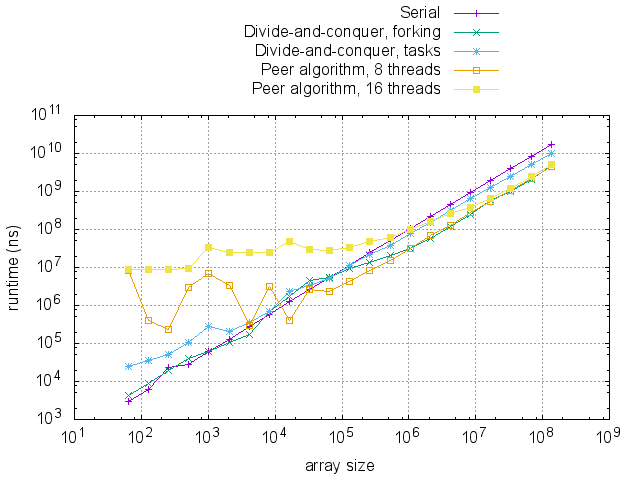
\includegraphics[width=0.75\textwidth]{plots/timings.png}
  \caption{Log-log of the timings of our programs for various array sizes.}
  \label{timings}
  \end{figure}

  \begin{figure}[h!]
  \centering
    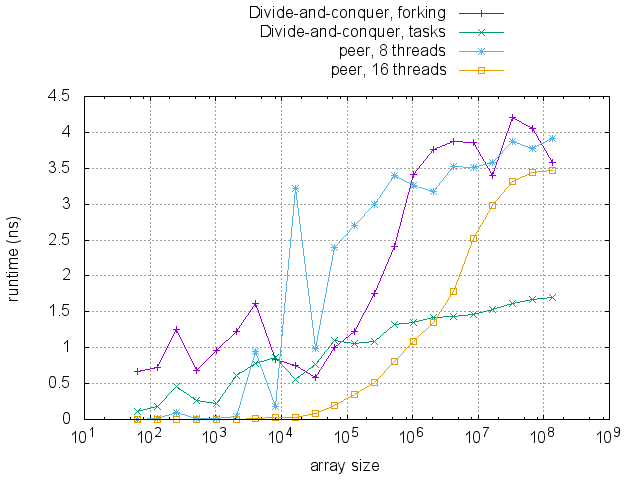
\includegraphics[width=0.75\textwidth]{plots/speedup.png}
  \caption{Log-log of the speedup of our programs for various array sizes.}
  \label{speedup}
  \end{figure}

\section{Conclusion}
  At the moment, the Divide-and-conquer method (where we spawn a lot of threads), works best.
  However, I still have faith that this implementation could be beaten by making more efficient use of the different threads by using a hybrid-model (do whatever leads to the best ratio of saturation vs. little-synchronization/context-switching) based on tasks. :)
\end{document}
